\section{Topological Phase Space}
In the last century, the development of modern physics has been partially driven by the incorporation of a few key concepts. A phase space is the spatial representation of all possible states of a dynamical system, where each point uniquely identifies a state. A Topological Phase Space can be defined as the n-dimensional spatial representation of the same using a generalized Curvilinear Coordinate system allowing for all possible coordinate transformations and perfect isometric compressions while preserving geometric invariance.

The concept of Phase Space in itself is a simple but powerful idea that emerged in the second half of the 19th century, during the golden era of differential geometry, and it is at the core of modern classical, quantum, and statistical mechanics. The trajectory that a dynamical system describes in the phase space as it evolves with time contains rich information about the system. For instance, by looking at the shape of the trajectories that a pendulum describes in its phase space, we can infer the existence of different dynamical regimes, or the ratio between the length of the pendulum and the acceleration of gravity.

The phase space of a simple pendulum is a two-dimensional cylinder, where the periodic coordinate corresponds to the angle (q) of the pendulum with respect to the vertical, and the longitudinal coordinate to its angular velocity (v). Each point in this space specifies a unique combination of the position and velocity and uniquely determines the subsequent evolution. For small angular velocities, the pendulum oscillates back and forth around the equilibrium point. For large velocities, the pendulum describes a circular motion. 

\begin{figure}[H]
  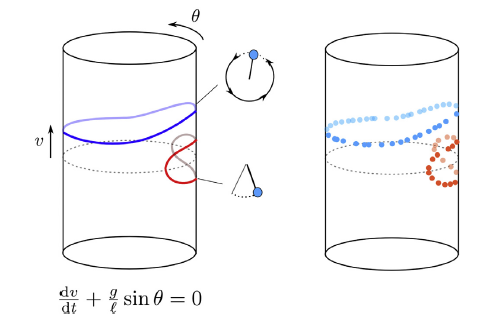
\includegraphics[width=\linewidth]{images/phase}
  \caption{Pendulum in Phase Space} % Figure caption
  \label{pendulum} 
\end{figure}

These two regimes are represented by qualitatively different trajectories in the phase space which cannot be continuously deformed into each other (in mathematical terms, they are homotopically inequivalent). By just looking at the shape of the trajectories in the phase space, we can extract information about a dynamical system. The dynamics of the simple pendulum is fully described by a differential equation depending on the length of the pendulum (l) and the acceleration of gravity (g). In more complex biological systems for example, such mathematical equations describing trajectories in the phase space are usually unknown, but current technologies allow to reconstruct trajectories from high-throughput measurements.



